\chapter[Metodologia]{Metodologia}
\label{cap:metodologia}

Este capítulo aborda a metodologia do trabalho, que foi utilizada para o desenvolvimento teórico e 
prático do mesmo. No primeiro momento, será abordada a Classificação da Pesquisa (\ref{section:classificacao_pesquisa}), considerando a 
Abordagem (\ref{section:classificacao_abordagem}), a Natureza (\ref{section:classificacao_natureza}), os Objetivos (\ref{section:classificacao_objetivos}) e os 
Procedimentos (\ref{section:classificacao_procedimentos}) da pesquisa. Na sequência, serão abordadas as 
metodologias que fundamentam este trabalho, em sua parte teórica e prática, sendo elas: Metodologia Investigativa (\ref{section:metod_investigativa}), 
Metodologia Orientada a Provas de Conceito (\ref{section:metod_poc}), Metodologia de Desenvolvimento (\ref{section:metodologia_desenvolvimento}) e 
Metodologia de Análise de Resultados (\ref{section:metodologia_analise_resultados}). 
Além disso, também será apresentado o Fluxo de Atividades/Subprocessos (\ref{section:fluxo_atividades}) 
e o Cronograma de Atividades/Subprocessos (\ref{section:cronograma}), que 
descrevem o escopo e as atividades definidas para a primeira e segunda etapa do TCC.
Por último, será apresentado o Resumo do Capítulo (\ref{section:resumo_metodologia}), recapitulando as seções abordadas neste capítulo.


\section{Classificação da Pesquisa}
\label{section:classificacao_pesquisa}

De acordo com \citeauthoronline{gerhardt2009metodos} (\citeyear{gerhardt2009metodos}), a pesquisa científica é a atividade principal da Ciência. Ela utiliza de 
métodos científicos de forma sistemática para explicar ou solucionar problemas. 
Os autores \citeauthoronline{gerhardt2009metodos} (\citeyear{gerhardt2009metodos}), ainda 
classificam uma pesquisa em quatro termos, sendo eles: abordagem, natureza, objetivos e procedimentos.

\subsection{Abordagem}
\label{section:classificacao_abordagem}

A abordagem de pesquisa deste trabalho pode ser classificada como \textbf{qualitativa} e \textbf{quantitativa}. 
A abordagem qualitativa tem o objetivo de aprofundar o conhecimento sobre um tema, utilizando de dados não-métricos, 
logo, ela não busca quantificar valores mas sim explicar o porquê das coisas através destes dados . 
Em contrapartida, a abordagem quantitativa busca quantificar seus resultados, através da análise de dados 
brutos que são coletados por ferramentas sistemáticas e neutras \cite{gerhardt2009metodos}.

Este trabalho busca analisar e quantificar dados brutos que podem ser coletados através da ferramenta SonarQube, 
sendo eles, quantidade de \textit{bugs}, complexidade ciclomática, segurança do código,  etc. Porém, além desta análise 
quantitativa, o trabalho também busca uma abordagem qualitativa ao analisar dados não-métricos, como por exemplo, o 
desempenho da aplicação após a reengenharia do código fonte em comparação com o projeto original.

\subsection{Natureza}
\label{section:classificacao_natureza}

Este trabalho pode ter sua natureza classificada como uma \textbf{pesquisa aplicada}. Este tipo de 
pesquisa busca gerar conhecimentos a partir de uma aplicação prática, e assim, solucionar problemas 
específicos \cite{gerhardt2009metodos}. A aplicação prática deste trabalho busca responder as 
questões levantadas nas Questões de Pesquisa e de Desenvolvimento (\ref{section:questoesdepesquisa}).

\subsection{Objetivos}
\label{section:classificacao_objetivos}

Este trabalho tem seus objetivos classificados no grupo da \textbf{pesquisa exploratória}. 
Esta pesquisa exploratória tem o intuito de trazer uma maior familiaridade com o problema, 
a fim de o tornar mais compreensível ou de formular hipóteses a partir dele \cite{gerhardt2009metodos}. Esta abordagem de objetivos 
está alinhada com o problema descrito na seção de Justificativa (\ref{section:justificativa}) do trabalho.

\subsection{Procedimentos}
\label{section:classificacao_procedimentos}

Em relação aos procedimentos deste trabalho, pode-se citar a \textbf{pesquisa bibliográfica}, 
definida pelos autores \citeauthoronline{gerhardt2009metodos} (\citeyear{gerhardt2009metodos}), 
que consiste no levantamento de referências teóricas já publicadas no meio científico, como artigos e livros, 
a fim de conhecer o que já foi estudado sobre o tema. Esta pesquisa compõe a Metodologia Investigativa (\ref{section:metod_investigativa}) do trabalho.

Este trabalho também conta com uma pesquisa de \textbf{provas de conceito}, que compõe a Metodologia Orientada a Provas de Conceito (\ref{section:metod_poc}). 
Com essa abordagem, é possível descrever desafios que evidenciam as 
capacidades de um \textit{software}, e verificam se o mesmo está cumprindo as necessidades dos clientes e usuários \cite{prasanna2021poc}.


\section{Metodologia Investigativa}
\label{section:metod_investigativa}

De acordo com \citeauthoronline{gil2002elaborar} (\citeyear{gil2002elaborar}), 
um trabalho científico inicia-se com uma pesquisa bibliográfica, 
que permite com que os autores conheçam o tema, que já foi definido, por meio de fontes 
científicas que já o abordaram antes. Assim, após a definição do tema deste trabalho, realizou-se 
um levantamento teórico na base científica Google Scholar, que é uma base consolidada, que permite 
a busca não só em artigos, mas também em livros, revistas e outras fontes científicas, fornecendo 
uma busca mais abrangente. A Tabela \ref{tab:strings_busca_tcc1} contém as \textit{strings} de busca que foram utilizadas 
neste levantamento, assim como a quantidade de fontes retornadas.


\begin{table}[h]
  \centering
  \caption{\textit{Strings} de busca}
  \begin{tabularx}{\linewidth}{l*{5}{>{\centering\arraybackslash}X}}
      \toprule
      \textbf{Base de dados} & \textbf{\textit{String}} & \textbf{Quantidade} \\
      \midrule
      \rowcolor{gray!20} Google Scholar & 'reverse engineering' & 4.610.000 \\
      Google Scholar & 'reengineering' & 414.000 \\
      \rowcolor{gray!20} Google Scholar & 'test-driven development (TDD)' & 13.500 \\
      Google Scholar & 'mobile development' & 5.940.000 \\
      \rowcolor{gray!20} Google Scholar & 'software design' & 8.900.000 \\
      Google Scholar & 'reengineering' AND 'reverse engineering' & 60.500 \\
      \rowcolor{gray!20} Google Scholar & 'reengineering' AND 'TDD' OR 'DDD' & 3.300 \\
      Google Scholar & 'TDD' AND 'DDD' & 11.000 \\
      \rowcolor{gray!20} Google Scholar & 'software design' AND 'mobile development' & 4.740.000 \\
      Google Scholar & 'TDD' AND 'DDD' & 11.000 \\
      \bottomrule
  \end{tabularx}
  \parbox{\linewidth}{\centering FONTE: Autores}
  \label{tab:strings_busca_tcc1}
\end{table}

\subsection{Critérios de Seleção}

A fim de filtrar as principais fontes a partir do material obtido no levantamento bibliográfico, 
tornou-se necessário realizar uma análise exploratória. Essa análise foi feita pelos autores,
a partir da leitura do resumo e das palavras-chave dos trabalhos, 
seguindo os seguintes critérios de seleção:

\begin{itemize}
  \item Abordar engenharia reversa no contexto da \textit{Engenharia de Software};
  \item Abordar reengenharia de \textit{software};
  \item Abordar desenvolvimento utilizando a técnica TDD e/ou orientado ao DDD, e
  \item Disponíveis gratuitamente.
\end{itemize}

Houve uma certa dificuldade em refinar o material obtido na Tabela \ref{tab:strings_busca_tcc1} com os 
critérios de seleção definidos. Esta dificuldade pode ser explicada primeiramente 
pelo fato dos temas de Engenharia Reversa e Reengenharia não serem exclusivos da 
Engenharia de \textit{Software}. Muitas fontes os abordam em contextos da manufatura e de 
outras áreas, não se relacionando com o contexto deste trabalho,  de utilizar estas práticas 
em um produto de \textit{software} já existente.

Outra dificuldade encontrada foi a falta de exemplos práticos da utilização da técnica de 
programação TDD juntamente com o desenvolvimento orientado ao DDD. Embora ambos tenham uma 
alta popularidade na comunidade de \textit{software}, eles não se tratam de uma associação 
óbvia, por atacarem áreas distintas de um produto de \textit{software} (testes e domínio).

As dificuldades encontradas foram contornadas por meio da alta quantidade de materiais retornados 
pelas \textit{strings} de busca definidas na Tabela \ref{tab:strings_busca_tcc1}, o que tornou possível o refinamento 
dos resultados obtidos e a seleção de fontes para compor a base bibliográfica deste trabalho. 
Os trabalhos escolhidos são:

\begin{itemize}
  \item \textit{Test driven development: By example} \cite{beck2022test};
  \item \textit{Implementing domain-driven design} \cite{vernon2013implementing};
  \item \textit{Refactoring} \cite{fowler2018refactoring};
  \item \textit{Design principles and design patterns} \cite{martin2000design}, e
  \item \textit{Reverse engineering and design recovery: A taxonomy} \cite{chikofsky1990reverse}.
\end{itemize}

Adicionalmente, torna-se necessário um outro estudo, que busca atender aos desafios definidos nas provas de conceito. 
O processo investigativo deste estudo é o mesmo que foi realizado anteriormente, 
seguindo os mesmos passos de pesquisa bibliográfica. Este subprocesso pode ser visto na 
Figura \ref{metodologia_investigativa}, que ilustra, utilizando a modelagem BPMN, as atividades presentes na metodologia investigativa.

% TODO: REVISAR TODAS AS TABELAS E FIGURAS PARA ADICIONAR TITULO E AUTOR
\begin{figure}[h]
    \caption{Fluxograma da Metodologia Investigativa}
	\centering
	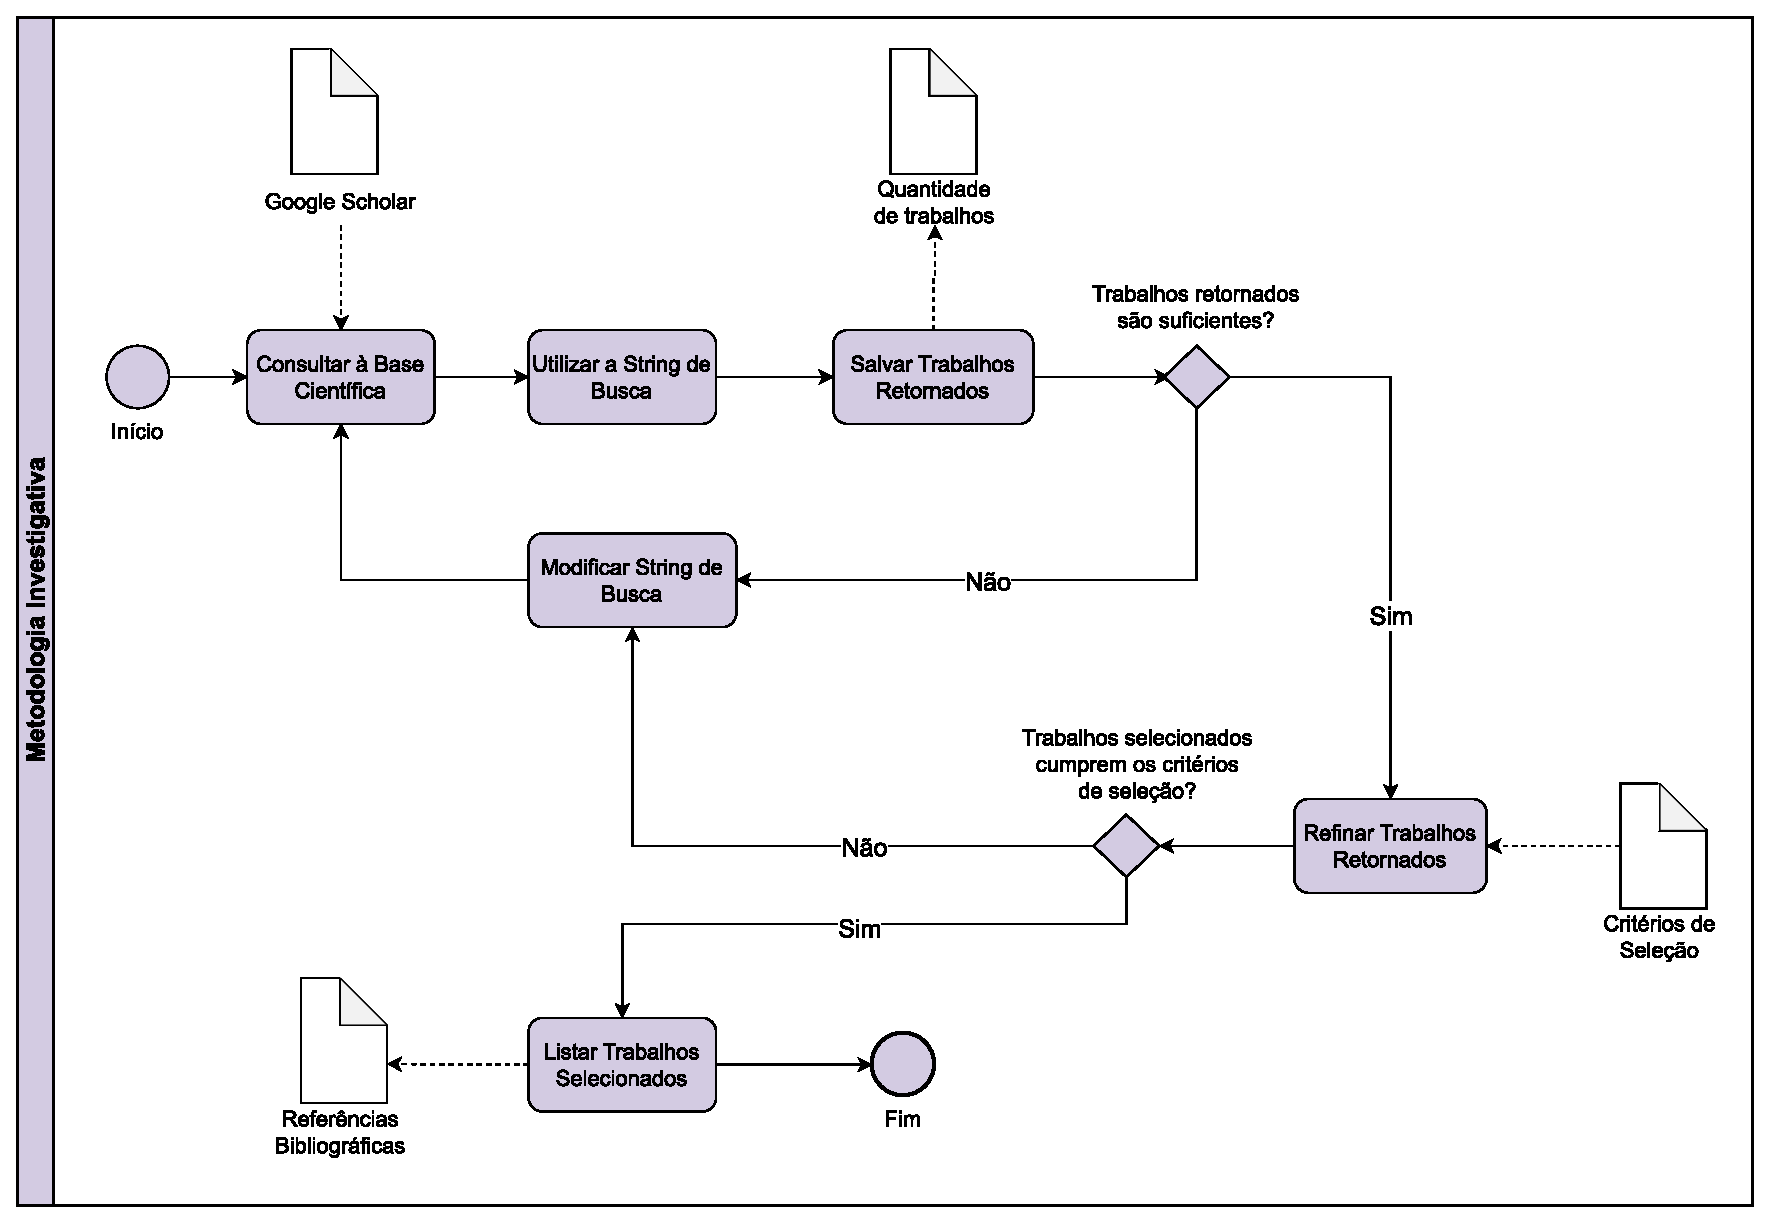
\includegraphics[keepaspectratio=true,scale=0.55]{figuras/metodologia_investigativa.eps}
    \parbox{\linewidth}{\centering FONTE: Autores}
	\label{metodologia_investigativa}
\end{figure}

\section{Metodologia Orientada a Provas de Conceito}
\label{section:metod_poc}

No contexto do desenvolvimento de \textit{software}, o termo Prova de Conceito (em inglês, 
\textit{Proof of Concept} - POC), é uma ferramenta que pode ser utilizada para demonstrar as 
capacidades de um \textit{software}, assim como sua viabilidade e se o mesmo atende as necessidades 
dos clientes e dos usuários. As provas de conceito podem ser aplicadas em diversas áreas, como 
\textit{marketing} e medicina. Já no domínio da \textit{Engenharia de Software}, elas seguem um 
processo específico que pode utilizar o desenvolvimento de \textit{hardware}, \textit{websites} ou 
outro tipo de \textit{software} que implemente um conceito \cite{prasanna2021poc}.

Nesta metodologia, o primeiro passo é estabelecer uma etapa inicial, também chamada 
de Definição do Desafio. Esta etapa possui o objetivo de fornecer uma compreensão clara do desafio 
que será abordado na prova de conceito, e pode ser feita por meio exclusivo de elementos textuais,  
ou também pode ser complementada com imagens e códigos fonte de exemplo \cite{silva2023microfrontends}.

Em seguida, vem a etapa do Estudo da Literatura, que tem o objetivo de fundamentar a solução para 
o desafio proposto por meio do embasamento teórico. Nesta etapa, é feito um estudo investigativo, 
com um olhar teórico e técnico, a fim de levantar conceitos e tecnologias adequadas para a futura 
solução, de forma que a mesma possua muita coerência e solidez \cite{silva2023microfrontends}.

Com o Estudo da Literatura realizado e pronto para fundamentar a solução, é possível realizar a 
apresentação da mesma. Na etapa de Apresentação da Solução, são utilizados elementos ilustrativos, 
como imagens, códigos fonte e outros elementos, a fim de fornecer mais clareza para expor esta 
solução. Uma solução deve atender o desafio proposto de forma satisfatória, não tendo a responsabilidade 
de o resolver de forma completa e definitiva, mas sim seguir as orientações definidas pela literatura 
especializada \cite{silva2023microfrontends}.

Após a apresentação da solução, faz-se necessário a realização de uma análise profunda e objetiva dos 
resultados obtidos, através da etapa de Análise de Resultados, podendo esta ser conduzida de maneira 
qualitativa ou quantitativa. No contexto qualitativo, recorre-se às percepções adquiridas pelo programador 
e/ou especialista ao longo do tempo. No contexto quantitativo os insumos métricos advindos de ferramentas 
de coleta de dados, como o SonarQube, podem ser utilizados. Esta etapa de análise tem o objetivo evidenciar 
os pontos positivos e negativos percebidos durante o processo \cite{silva2023microfrontends}.

Na literatura, existem diversas abordagens metodológicas para as provas de conceito, o que torna uma 
escolha livre para os pesquisadores qual dessas abordagens adotar para o trabalho. Neste trabalho, a 
abordagem metodológica escolhida está definida em \citeauthoronline{turilli2016designing} (\citeyear{turilli2016designing}), 
que define uma metodologia sequencial 
para as provas de conceito. Com isso, uma próxima prova de conceito depende do sucesso da prova realizada 
anteriormente, sendo assim, uma orientação em \textit{Building Blocks}.

De acordo com \citeauthoronline{turilli2016designing} (\citeyear{turilli2016designing}), o 
conceito de \textit{Building Blocks}, assim como o nome sugere, é a 
realização da prova de conceito por meio de blocos de construção, que são etapas que devem ser executadas 
de maneira sequencial. Esta abordagem busca reduzir um grande problema em pequenos módulos mais 
compreensíveis. Ao utilizar este conceito, os autores buscam reduzir o tema proposto, que possui uma 
certa complexidade, em desafios menores utilizando as provas de conceito.

Ao utilizar as etapas definidas por esta metodologia (Definição do Desafio, Estudo da Literatura, 
Apresentação da Solução e Análise de Resultados), juntamente com o conceito dos \textit{Building Blocks}, 
é possível realizar o estudo exploratório deste trabalho. As provas de conceito serão realizadas de forma 
sequencial, podendo ter ajustes pontuais e justificados caso alguma das provas não seja concluída com 
sucesso. A Figura \ref{metodologia_poc} ilustra, por meio da modelagem BPMN, as etapas da Metodologia Orientada a Provas de Conceito.

\begin{figure}[h]
	\centering
    \caption{Fluxograma da Metodologia Orientada a Provas de Conceito}
	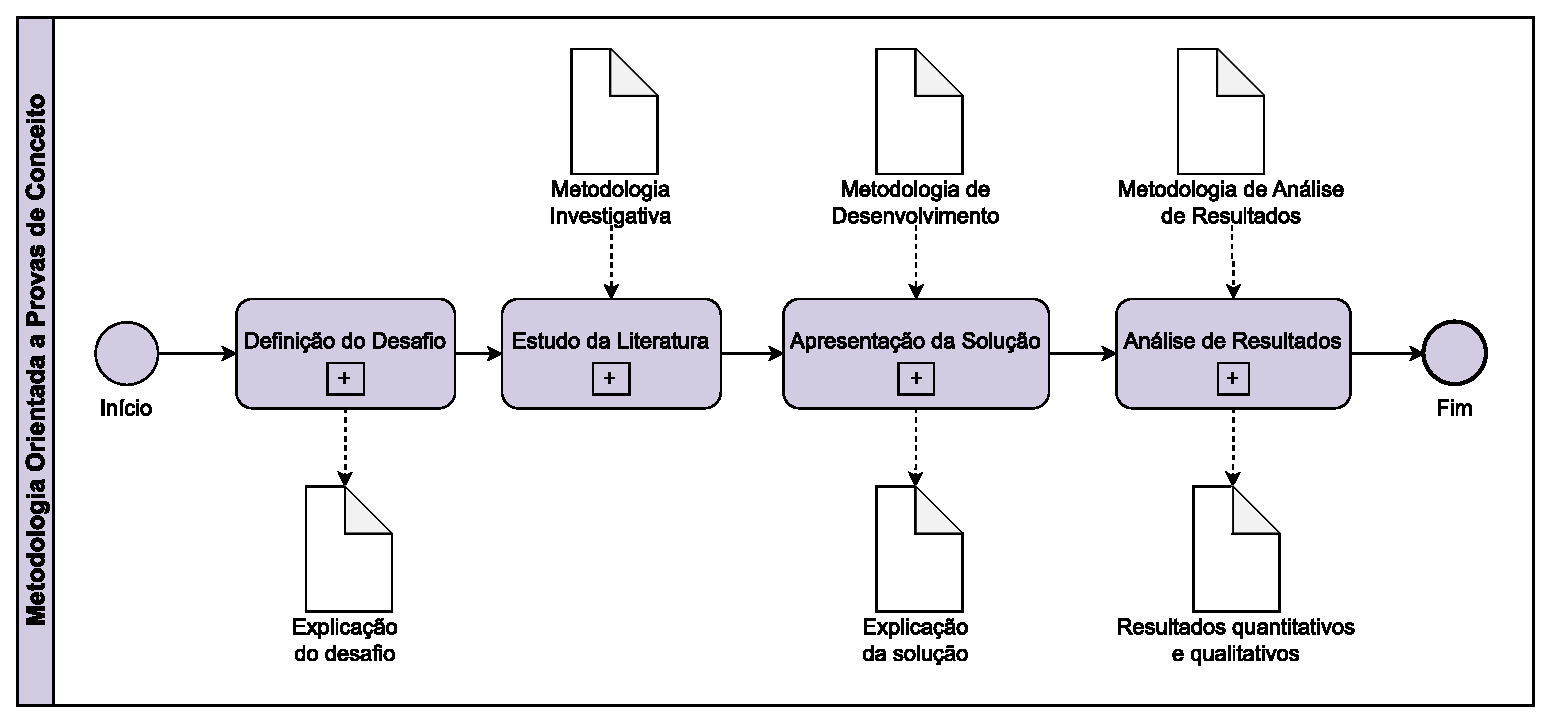
\includegraphics[keepaspectratio=true,scale=0.6]{figuras/metodologia_poc.eps}
    \parbox{\linewidth}{\centering FONTE: Autores}
	\label{metodologia_poc}
\end{figure}

\section{Metodologia de Desenvolvimento}
\label{section:metodologia_desenvolvimento}

A metodologia empregada no desenvolvimento prático deste trabalho será híbrida, 
fundamentada na combinação dos principais elementos das metodologias ágeis Scrum \cite{sutherland2014scrum} 
e o Kanban \cite{ahmad2013kanban}, considerando a sua relevância no atual cenário de 
mercado e desenvolvimento de \textit{software} \cite{carvalho2012aplicaccao}.

O Scrum apresenta diversas características individuais, como reuniões diárias, de planejamento 
e retrospectivas, além da definição de papéis e responsabilidades dos membros da equipe durante 
o processo de desenvolvimento de um produto  \cite{sutherland2014scrum}. No entanto, opta-se 
por uma abordagem mais sutil e simplificada em relação ao Scrum clássico, priorizando o uso 
do \textit{Product Backlog} como principal ferramenta, combinando com práticas do Kanban e dispondo 
as tarefas no Trello.

A construção do \textit{Product Backlog} envolve a especificação do projeto em diversos níveis 
de granularidades, incluindo Épicos, \textit{Features}, \textit{User Stories}, Tarefas e Critérios de 
Aceitação, onde tudo o que é definido no \textit{backlog} deve agregar valor ao produto. A partir 
dessa definição, são iniciadas várias iterações dentro do processo de desenvolvimento, conhecidas 
como \textit{sprints}. As \textit{sprints} são períodos de tempo curtos e bem definidos pelos times 
para o desenvolvimento das tarefas do \textit{backlog} \cite{sutherland2014scrum}.

Como mencionado anteriormente, o uso do Kanban será de extrema relevância para o desenvolvimento deste 
trabalho. O Kanban é uma prática que tem como objetivo visualizar, de forma facilitada, o andamento do processo de 
desenvolvimento de um produto. Além de facilitar o gerenciamento das tarefas, indica o \textit{status}, o responsável 
por determinada tarefa e limita a quantidade que cada integrante da equipe pode realizar.

Dessa forma, a metodologia de desenvolvimento prático desse trabalho será baseada, principalmente em:

\begin{itemize}
    \item Definição do \textit{Backlog}: Nessa etapa será desenvolvido todo o \textit{backlog} de 
    tarefas que serão cumpridas até o final do cronograma definido. Todas as tarefas serão iniciadas 
    com o \textit{status} \textit{ToDo}, inicialmente seguindo o Kanban \cite{ahmad2013kanban};
    \item Desenvolvimento da Tarefa: Nessa etapa, as tarefas que foram selecionadas para serem desenvolvidas 
    dentro da \textit{sprint} serão distribuídas entre os integrantes. O \textit{status} será alterado 
    para \textit{Doing} no momento em que o respectivo integrante der início ao desenvolvimento da tarefa. 
    O \textit{status} é, novamente, alterado para \textit{Done} novamente quando a tarefa for finalizada com 
    a possibilidade de seguir com o desenvolvimento de uma nova tarefa ou retornar para a revisão de uma 
    tarefa já finalizada, e
    \item Revisão de Tarefa: Nessa etapa é feito o envio das tarefas para avaliação por parte da equipe do 
    projeto (autores e orientadores). No caso de aprovação da tarefa, o \textit{status} da mesma é alterado 
    para \textit{Reviewed}. Caso seja necessária alguma alteração, a tarefa retornará para desenvolvimento, 
    assim como seu \textit{status} que será alterado para \textit{Doing} novamente.
\end{itemize}

A Figura \ref{flux_dev} mostra o fluxo detalhado do processo descrito anteriormente, resumindo 
a Metodologia de Desenvolvimento.

\begin{figure}[h]
	\centering
    \caption{Fluxograma de Desenvolvimento}
	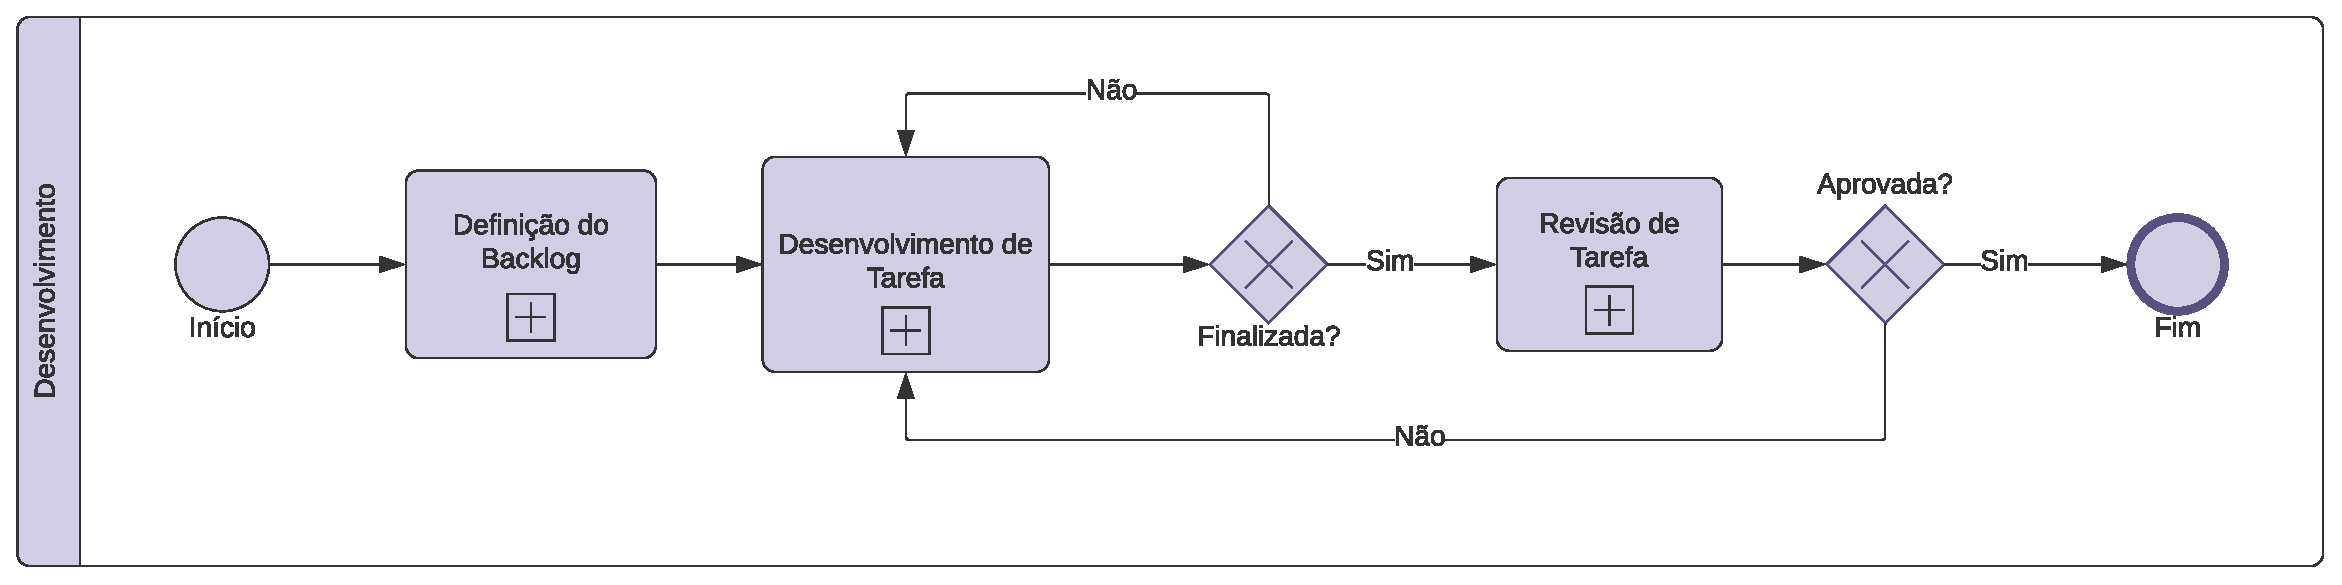
\includegraphics[keepaspectratio=true,scale=0.4]{figuras/fluxo_desenvolvimento.eps}
	\parbox{\linewidth}{\centering FONTE: Autores}
	\label{flux_dev}
\end{figure}

É importante ressaltar que a metodologia de desenvolvimento, descrita nessa seção, será utilizada juntamente 
com a Metodologia Orientada a Provas de Conceito, item \ref{section:metod_poc}.

\section{Metodologia de Análise de Resultados}
\label{section:metodologia_analise_resultados}

A pesquisa de campo é caracterizada por investigações que vão além da pesquisa bibliográfica e/ou documental, 
envolvendo a coleta de dados junto a pessoas por meio de diferentes tipos de pesquisa, como, por exemplo, \textit{ex-post-facto}, 
pesquisa-ação e pesquisa participante \cite{gerhardt2009metodos}. Ainda segundo \cite{gerhardt2009metodos}, com o propósito 
de analisar os resultados obtidos durante o desenvolvimento do trabalho, a metodologia adotada será a pesquisa-ação, 
fundamentada na resolução de questões ou problemas por meio da investigação. Nesse método, os pesquisadores participam de 
forma colaborativa ou participativa. \cite{thiollent1988metodologia} explica:

\begin{quotation}
\begin{adjustwidth}{4cm}{-1cm}
"A pesquisa ação é um tipo de investigação social com base empírica que é concebida e realizada em estreita 
associação com uma ação ou com a resolução de um problema coletivo no qual os pesquisadores e os participantes representativos 
da situação ou do problema estão envolvidos de modo cooperativo ou participativo (p. 14)."
\end{adjustwidth}
\end{quotation}

Enquanto \cite{da2002apostila} define por:

\begin{quotation}
\begin{adjustwidth}{4cm}{-1cm}
"A pesquisa-ação pressupõe uma participação planejada do pesquisador na situação problemática a ser investigada. O processo de pesquisa 
recorre a uma metodologia sistemática, no sentido de transformar as realidades observadas, a partir da sua compreensão, conhecimento e 
compromisso para a ação dos elementos envolvidos na pesquisa (p. 34). O objeto da pesquisa-ação é uma situação social situada em conjunto 
e não um conjunto de variáveis isoladas que se poderiam analisar independentemente do resto. Os dados recolhidos no decurso do trabalho 
não têm valor significativo em si, interessando enquanto elementos de um processo de mudança social. O investigador abandona o papel 
de observador em proveito de uma atitude participativa e de uma relação sujeito a sujeito com os outros parceiros. O pesquisador quando 
participa na ação traz consigo uma série de conhecimentos que serão o substrato para a realização da sua análise reflexiva sobre a 
realidade e os elementos que a integram. A reflexão sobre a prática implica em modificações no conhecimento do pesquisador (p. 35)."
\end{adjustwidth}
\end{quotation}

O objetivo principal desse método de pesquisa é examinar as características de diversos métodos disponíveis, avaliando suas capacidades, 
potencialidades, limitações ou distorções, além de identificar os pressupostos ou implicações de sua aplicação. Em um nível mais prático, 
envolve a avaliação de técnicas de pesquisa e a geração ou experimentação de novos métodos relacionados aos modos eficazes de coletar e 
processar informações. Além disso, busca solucionar diversas categorias de problemas teóricos e práticos na pesquisa, servindo como uma 
maneira de conceber e organizar o objeto de pesquisa, conforme alinnhado por \cite{thiollent1988metodologia}.

A metodologia de pesquisa-ação possui particularidades para cada pesquisa, dependendo de sua demanda. No desenvolvimento 
desse trabalho, optou-se por direcionar a metodologia da seguinte maneira:

\begin{itemize}
    \item Levantamento Investigativo: Nessa etapa, o foco principal é a obtenção de informações relevantes e 
    significativas visando justificar a elaboração da pesquisa. Dessa forma, foi realizada uma Pesquisa Bibliográfica, 
    já descrita anteriormente em Metodologia Investigativa, no Tópico \ref{section:metod_investigativa}, cujos resultados estão documentados nos 
    Capítulos \ref{cap:referencial} e \ref{cap:suporte} de Referencial Teórico e de Suporte Tecnológico, respectivamente. 
    Adicionalmente, conduziu-se uma análise cuidadosa de documentos disponíveis para extrair informações pertinentes;

    \item Planejamento: Nesta etapa, delineiam-se claramente os objetivos da pesquisa, indicando o que se espera alcançar. 
    Além disso, foram elaboradas as questões de pesquisa que norteiam o presente trabalho, conforme discutido no Capítulo 
    \ref{cap:introducao}. A seleção de métodos e técnicas foi desenvolvida com o objetivo de orientar as atividades ao longo 
    do tempo, sem excluir a possibilidade de adequações conforme a demanda; 

    \item Ação: Com o plano de pesquisa definido, passa-se à implementação efetiva das ações planejadas. Isso inclui a aplicação dos 
    métodos e técnicas selecionados, bem como a coleta adicional de dados, se necessário. Durante essa fase, são registradas observações 
    detalhadas para documentar o progresso e os \textit{insights} obtidos \cite{krafta2007metodo}, e
    
    \item Avaliação: Nessa etapa é realizada a análise crítica dos resultados obtidos. Isso envolve examinar os dados coletados, 
    verificando se as hipóteses foram confirmadas ou refutadas e refletir criticamente sobre o processo de pesquisa. Com base nessa 
    análise, são elaboradas conclusões sólidas que resumem os resultados e, se necessário, identificam-se áreas para melhorias 
    futuras \cite{furtado2008avaliaccao}.
\end{itemize}

\section{Fluxo de Atividades/Subprocessos}
\label{section:fluxo_atividades}

Durante a execução deste estudo, estabeleceram-se metas para otimizar a consecução do resultado desejado na primeira fase, que consiste 
na entrega do TCC1. Visando assegurar a conclusão integral desta pesquisa, elaborou-se um fluxograma abrangente que contempla não apenas 
as etapas atuais (Figura \ref{fluxograma_atividades_tcc1}), mas também aquelas planejadas para a segunda fase, referente à entrega do TCC2. 
As Figuras \ref{fluxograma_atividades_tcc1} e \ref{fluxograma_atividades_tcc2} apresentam os fluxos delineados para a realização das 
etapas necessárias nas entregas do TCC1 e TCC2, respectivamente.

\subsection{Primeira Etapa do TCC}

\begin{figure}[h]
	\centering
    \caption{Fluxograma de Atividades/Subprocessos do TCC1}
	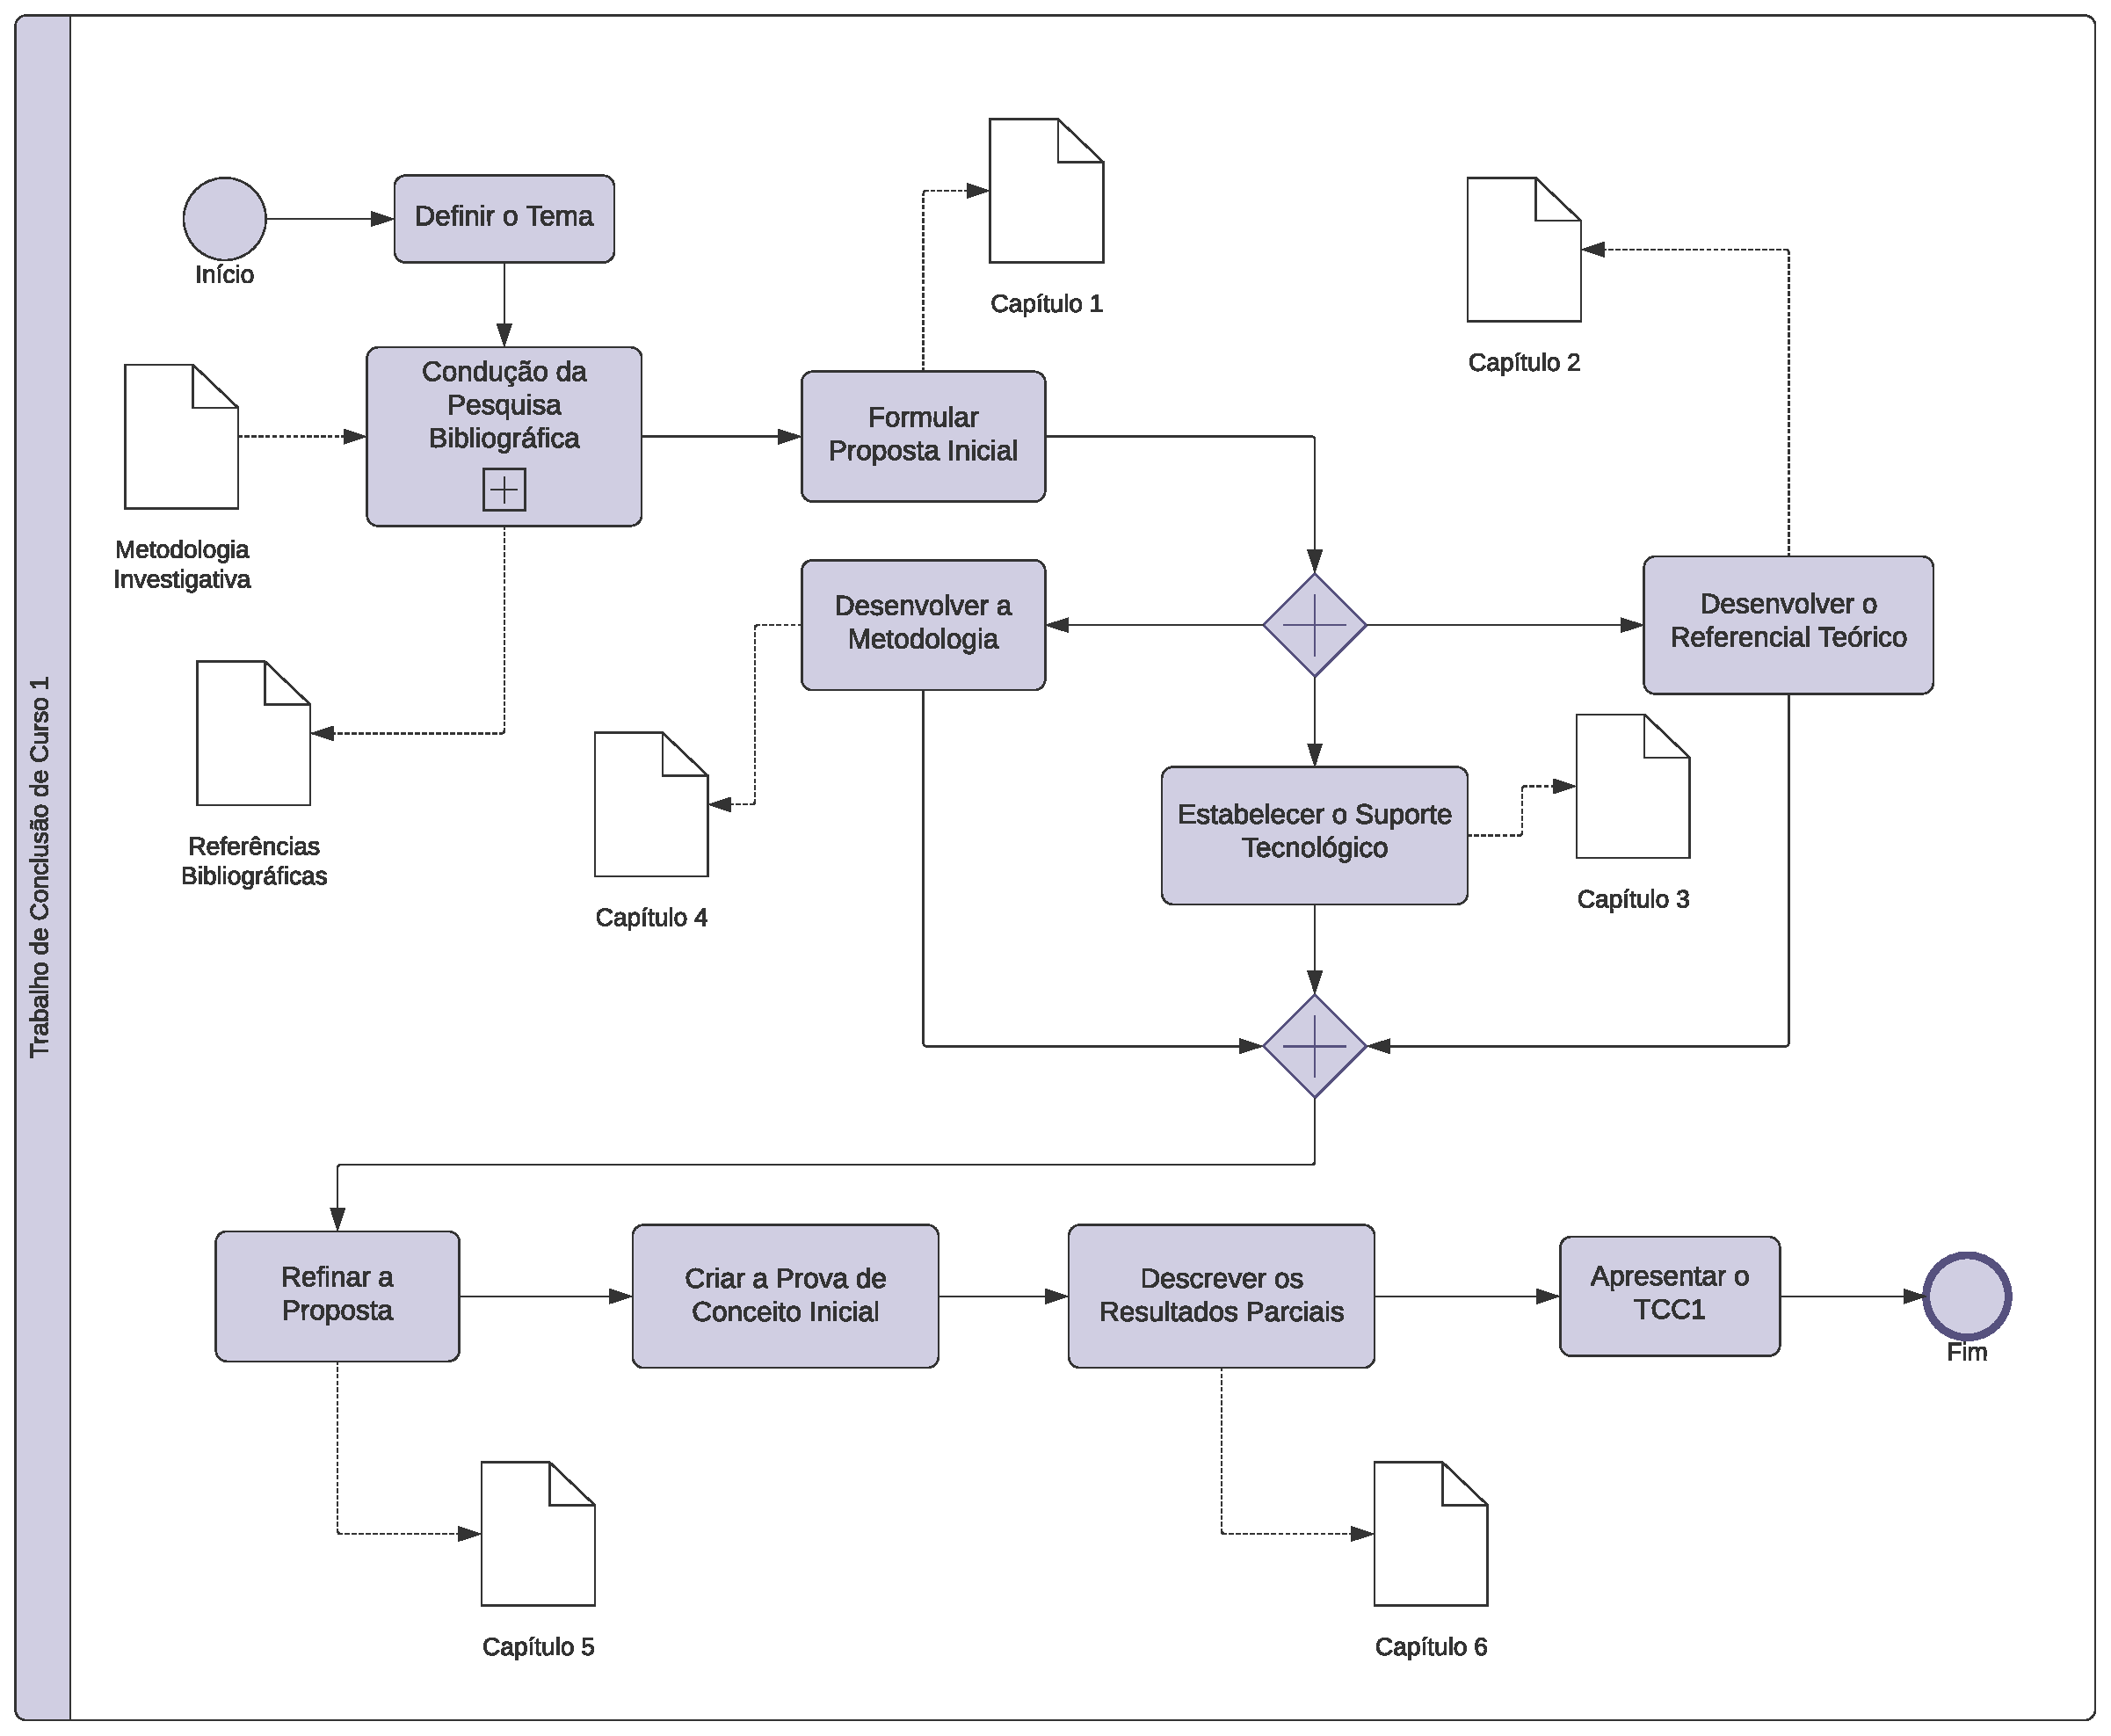
\includegraphics[keepaspectratio=true,scale=0.4]{figuras/fluxograma_atividades_tcc1.eps}
	\parbox{\linewidth}{\centering FONTE: Autores}
	\label{fluxograma_atividades_tcc1}
\end{figure}

1. \textbf{Definir o Tema:} Essa fase inicial visa discernir e delinear o tema central que guiará toda a pesquisa. A escolha do tema requer, ao menos,
uma compreensão mínima das lacunas no conhecimento existente e a capacidade de formular uma questão de pesquisa clara e significativa.
\textit{Status:} Concluída;

2. \textbf{Conduzir a Pesquisa Bibliográfica:} Essa fase envolve a condução de uma pesquisa bibliográfica abrangente, buscando não apenas a coleta de 
informações, mas também a análise crítica e a síntese de conhecimentos prévios. Este processo exige habilidades de discernimento, julgamento acadêmico e 
a capacidade de situar a pesquisa no contexto mais amplo do campo de estudo. Deve-se cumprir os critérios apresentados no item \ref{cap:introducao}, 
conforme bem destrinchado nos subitens \ref{section:questoesdepesquisa} e \ref{section:objetivos}.
\textit{Status:} Concluída;

3. \textbf{Formular a Proposta Inicial:} Nessa etapa, reforça-se que a formulação da proposta inicial não se restringe à articulação dos objetivos 
da pesquisa, sendo uma tarefa de contextualização do trabalho em relação às contribuições já existentes. Se demanda, aqui, a síntese de ideias e a 
comunicação eficaz, assegurando que a proposta seja robusta, inovadora e alinhada aos propósitos do estudo, conforme apresentado também no item \ref{cap:introducao}.
\textit{Status:} Concluída;

4. \textbf{Desenvolver o Referencial Teórico:} O desenvolvimento do referencial teórico vai além de compilar teorias, requerendo a síntese  
e a integração de conceitos fundamentais para o tema escolhido, como por exemplo: Reengenharia, Aplicativos Móveis, \textit{Test-Driven Development} (TDD), 
\textit{Domain-Driven Design} (DDD), Técnicas de Programação, dentre outros. Este processo exige separação de literatura relevante para o tema, conjutamente com a 
combinação de informações importantes associadas ao tema, conforme apresentado no item \ref{cap:referencial}.
\textit{Status:} Concluída;

5. \textbf{Estabelecer o Suporte Tecnológico:} Nessa etapa, foca-se na escolha de ferramentas, de modo a viabilizar a pesquisa, alinhando-as estrategicamente 
aos objetivos do estudo. A descrição dessas ferramentas - para desenvolvimento prático do trabalho - resultaram no item \ref{cap:suporte}.
\textit{Status:} Concluída;

6. \textbf{Desenvolver a Metodologia:} Nessa fase, a pesquisa avança para a elaboração de um plano prático, conforme descrito ao longo do presente capítulo 
(item \ref{cap:metodologia}). O objetivo visa definir os métodos e procedimentos que serão utilizados, assegurando uma metodologia eficiente, focando-se em uma 
obtenção confiável de resultados. 
\textit{Status:} Concluída;

7. \textbf{Refinar a Proposta:} Nessa fase, concentra-se os esforços no aprimoramento da proposta inicial com base em \textit{feedbacks} recebidos. O intuito é 
tornár o trabalho desenvolvido mais claro, relevante e inovador.
\textit{Status:} Concluída;

8. \textbf{Criar a Prova de Conceito Inicial:} Essa etapa envolve a tradução da proposta em algo tangível, como um protótipo ou versão preliminar. O objetivo é 
validar a viabilidade da abordagem proposta bem como a configuração de ambiente de desenvolvimento, conforme item no Capítulo 5.
\textit{Status:} Concluída;

9. \textbf{Descrever os Resultados Parciais:} Nessa fase, apresenta-se e analisa-se as descobertas obtidas até o momento (TCC1). A análise crítica para identificar 
resultados, destacando sua relevância em relação aos objetivos da pesquisa é necessária. Essa descrição parcial atua como um indicador do progresso, 
fornecendo \textit{insights} valiosos para orientar as próximas etapas (TCC2).
\textit{Status:} Concluída, e

10. \textbf{Apresentar o TCC1:} Etapa em que serão compartilhados os fundamentos teóricos, metodológicos e os resultados obtidos até momento para a banca examinadora.
\textit{Status:} Concluída;

\subsection{Segunda Etapa do TCC}

\begin{figure}[h]
	\centering
    \caption{Fluxograma de Atividades/Subprocessos do TCC2}
	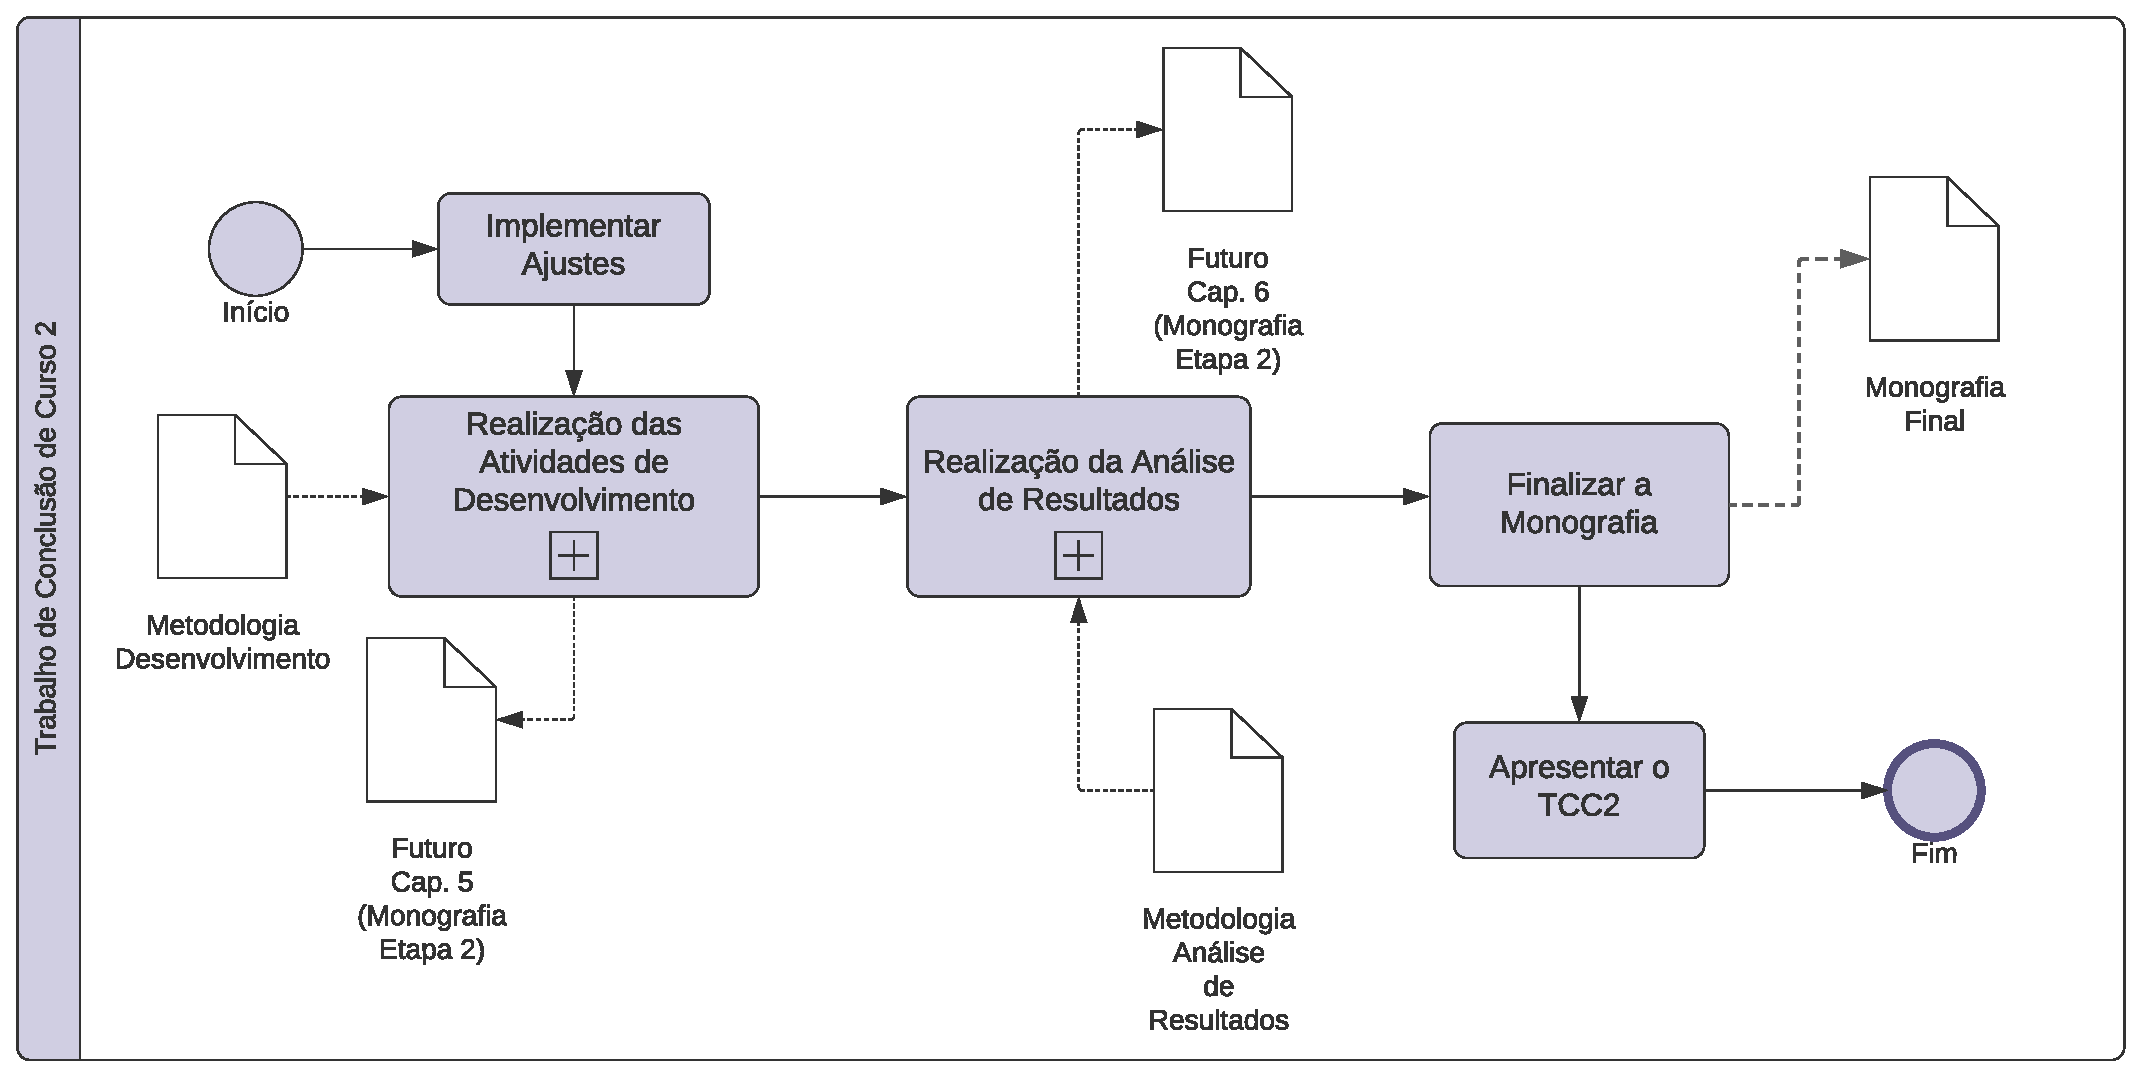
\includegraphics[keepaspectratio=true,scale=0.45]{figuras/fluxograma_atividades_tcc2.eps}
	\parbox{\linewidth}{\centering FONTE: Autores}
	\label{fluxograma_atividades_tcc2}
\end{figure}

1. \textbf{Implementar Ajustes:} Nessa etapa, procede-se à incorporação das modificações sugeridas pela banca avaliadora. Isso implica na revisão e adaptação do 
trabalho de acordo com as orientações recebidas, afim de se aprimorar a qualidade e a consistência do trabalho acadêmico. 
\textit{Status:} Concluída;

2. \textbf{Realização das Atividades de Desenvolvimento:} Essa etapa baseia-se na execução das atividades delineadas no Capítulo 5 - Proposta. A condução do 
desenvolvimento segue a Metodologia Orientada a Provas de Conceito (Tópico \ref{section:metod_poc}) e Metodologia de Desenvolvimento 
(Tópico \ref{section:metodologia_desenvolvimento}) como guias principais. Este processo enfoca a aplicação prática das diretrizes estabelecidas, 
assegurando a progressão coerente e eficaz do projeto.
\textit{Status:} Concluída;

3. \textbf{Realização da Análise de Resultados:} A condução dessa atividade segue os princípios e diretrizes estabelecidos pela Metodologia de Análise de Resultados, 
conforme tópico \ref{section:metodologia_analise_resultados}. O objetivo central é aplicar uma abordagem sistemática para interpretar e compreender os resultados 
obtidos, proporcionando \textit{insights} fundamentais para a finalização da pesquisa.
\textit{Status:} Concluída;

4. \textbf{Finalizar a Monografia:} Essa etapa representa o fechamento da monografia, fornecendo uma visão geral do estado final do trabalho. Durante esse processo, 
destaca-se os objetivos alcançados e o que pode ser explorado em futuras pesquisas referentes ao tema, indicando-se possíveis direções para investigações subsequentes.
\textit{Status:} Concluída, e

5. \textbf{Apresentar o TCC2:} Etapa em que serão compartilhados os fundamentos teóricos, metodológicos e os resultados obtidos para a banca examinadora.
\textit{Status:} Concluída.

\section{Cronograma de Atividades/Subprocessos}
\label{section:cronograma}

Com base nos fluxos previamente propostos, elaboraram-se os cronogramas correspondentes para a conclusão das fases inicial 
(Tabela \ref{tab:cronograma_tcc1}) e subsequente (Tabela \ref{tab:cronograma_tcc2}) deste trabalho.

\begin{table}[h]
    \centering
    \caption{Cronograma de atividades/subprocessos da primeira etapa do TCC}
    \begin{tabularx}{\linewidth}{l*{5}{>{\centering\arraybackslash}X}}
        \toprule
        \textbf{Atividades/Subprocessos} & \textbf{Ago} & \textbf{Set} & \textbf{Out} & \textbf{Nov} & \textbf{Dez} \\
        \midrule
        \rowcolor{gray!20} Definir o Tema & X & & & & \\
        Conduzir a Pesquisa Bibliográfica & X & & & & \\
        \rowcolor{gray!20} Formular a Proposta Inicial & & X & & & \\
        Desenvolver o Referencial Teórico & & & X & & \\
        \rowcolor{gray!20} Estabelecer o Suporte Tecnológico & & & X & & \\
        Desenvolver a Metodologia & & & & X & \\
        \rowcolor{gray!20} Refinar a Proposta & & & & & X \\
        Criar a Prova de Conceito Inicial & & & & & X \\
        \rowcolor{gray!20} Descrever os Resultados Parciais & & & & & X \\
        Apresentar o TCC1 & & & & & X \\
        \bottomrule
    \end{tabularx}
    \parbox{\linewidth}{\centering FONTE: Autores}
    \label{tab:cronograma_tcc1}
\end{table}

\begin{table}[h]
    \centering
    \caption{Cronograma de atividades/subprocessos da segunda etapa do TCC}
    \begin{tabularx}{\linewidth}{l*{5}{>{\centering\arraybackslash}X}}
        \toprule
        \textbf{Atividades/Subprocessos} & \textbf{Mar} & \textbf{Abr} & \textbf{Mai} & \textbf{Jun} & \textbf{Jul} \\
        \midrule
        Implementar Ajustes & X & & & & \\
        \rowcolor{gray!20} Realização das Atividades de Desenvolvimento & X & X & X & X &  \\
        Realização da Análise de Resultados & & & & X & X \\
        \rowcolor{gray!20} Finalizar a Monografia & & & & & X \\
        Apresentar o TCC2 & & & & & X \\
        \bottomrule
    \end{tabularx}
    \parbox{\linewidth}{\centering FONTE: Autores}
    \label{tab:cronograma_tcc2}
\end{table}

\section{Considerações Finais do Capítulo}
\label{section:resumo_metodologia}

Este capítulo teve o intuito de descrever a metodologia do trabalho, utilizada na sua confecção teórica e prática.
No primeiro momento, a pesquisa foi classificada da seguinte forma: de abordagem híbrida (qualitativa e quantitativa), 
de natureza aplicada, com objetivos exploratórios, e com procedimentos de caráter bibliográficos e orientados a provas de conceito.
Depois, o trabalho definiu seus elementos de pesquisa baseado na literatura científica. A partir disso, foram estabelecidas as seguintes
metodologias específicas: Metodologia Investigativa, para o desenvolvimento da pesquisa bibliográfica; Metodologia Orientada a Provas de Conceito, 
para a criação dos desafios práticos do trabalho; Metodologia de Desenvolvimento, que consiste numa abordagem híbrida, sendo fundamentada na combinação
de elementos das metodologias ágeis (Scrum e Kanban); e a Metodologia de Análise de Resultados, para a utilização da metodologia pesquisa-ação
que analisa os resultados obtidos. Por fim, o capítulo expôs fluxos de atividades e cronogramas para as duas etapas do TCC.